\chapter{Courbes paramétrées}

\sld{\includegraphics[width=\textwidth]{../figures/td4cinematique.png}}

\pl{Dans ce chapitre nous allons voir les propriétés fondamentales des courbes paramétrées.  Pour fixer les idées, commençons par présenter une courbe particulière: la \emph{cycloïde}. C'est la courbe que parcourt un point choisi de la roue d'un vélo, lorsque le vélo avance. Les coordonnées $(x,y)$ de ce point $M$ varient en fonction du temps:}
$$\left\{\begin{array}{rcl}
x(t) &=& r(t-\sin t) \\
y(t) &=& r(1-\cos t)
\end{array} \right.$$
où $r$ est le rayon de la roue.

\begin{center}
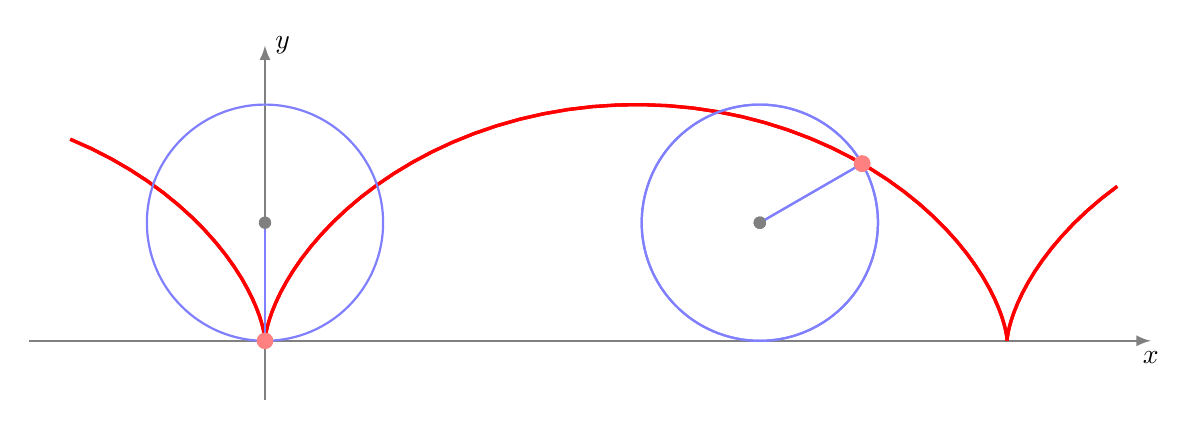
\begin{tikzpicture}[scale=1.5]

     \draw[->,>=latex,thick, gray] (-2,0)--(7.5,0) node[below,black] {$x$};
     \draw[->,>=latex,thick, gray] (0,-0.5)--(0,2.5) node[right,black] {$y$};

% Cycloide
\sld
\pl{
  \draw[red, very thick,domain=-0.75*pi:2.6*pi,samples=100] plot ({\x - sin(\x r)},{1 - cos(\x r)});
  }
\def\t{60}

\def\mkRoue#1#2{
\def\t{#1}
\begin{scope}[xshift=0.01745*\t cm, yshift=1 cm,rotate=-\t]
     \draw[thick, blue!#2]  (0,0) circle (1);
     \draw[thick, blue!#2] (0,0)--(0,-1);
     \fill[black!#2] (0,0) circle (1.5pt);
     \fill[red!#2] (0,-1) circle (2pt);
\end{scope}
}
\sld{%\uncover<1->}{
\mkRoue{0}{50};
%\mkRoue{80}{50};
\mkRoue{240}{50};
}

\pl{
\mkRoue{240}{50};
}
%\beameronly {\uncover<3->}{\mkRoue{160}{100};}

\end{tikzpicture}
\end{center}

La cycloïde a des propriétés remarquables. Par exemple, la cycloïde renversée est une courbe \emph{brachistochrone}: c'est-à-dire que c'est la courbe qui permet à une bille (soumis à la seule gravité) d'arriver le plus vite possible d'un point $A$ à un point $B$.  Contrairement à ce que l'on pourrait croire ce n'est pas une ligne droite, mais bel et bien un arc de cycloïde.  Sur le dessin suivant les deux billes sont lâchées en $A$ à l'instant $t_0$, l'une sur le segment $[AB]$ ; elle aura donc une accélération constante.  La seconde parcourt la cycloïde renversée, ayant une tangente verticale en $A$ et passant par $B$.  La bille accélère beaucoup au début et elle atteint $B$ bien avant l'autre bille (à l'instant $t_4$ sur le dessin).  Notez que la bille passe même par des positions en-dessous de $B$ (par exemple en $t_3$).  

\begin{center}

    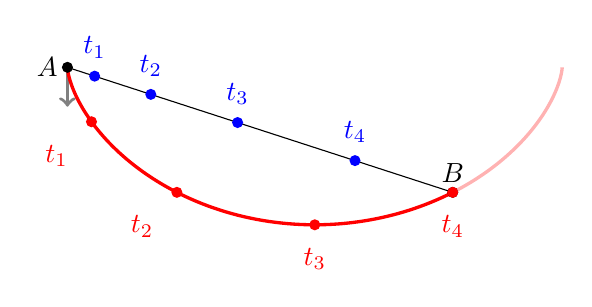
\begin{tikzpicture}
%
%      \draw[->,>=latex,thick, gray] (-2,0)--(3.5,0) node[below,black] {$x$};
%      \draw[->,>=latex,thick, gray] (0,-2.5)--(0,2.5) node[right,black] {$y$};

    %tangente à l'origine
        \draw[gray,very thick,->] (0,0) -- (0,-.5);
% Cycloide

        \def\T{1.3*pi};  % Do not change
        \def\a{\T-sin(deg(\T))};
        \def\b{-1+cos(deg(\T))};
        \draw (0,0)--({\a},{\b});


        \draw[red, very thick,domain=0:\T,samples=100] plot ({\x - sin(\x r)},{-1+ cos(\x r)});
        \draw[red!30, very thick,domain= \T:2*pi,samples=100] plot ({\x - sin(\x r)},{-1+ cos(\x r)});

% \def\x{4.08};
% \fill[black] ({\x - sin(\x r)},{-1+ cos(\x r)})circle (2pt) ;

        \fill[black] (0,0) circle (2pt) node[left] {$A$};
        \fill[black] ({\a},{\b}) circle (2pt) node[above] {$B$};


% Variables: time=angle, transparency, index, position index
        \def\mkPlot#1#2#3#4{
            \def\t{#1}

   % Cycloide
            \def\newa{\t-sin(deg(\t))};
            \def\newb{-1+cos(deg(\t))};
            \fill[red!#2] ({\newa},{\newb}) circle (2pt) node[#4=5pt] {$t_{#3}$};

  % Line
            \def\r{sqrt((\a)*(\a)+(\b)*(\b))};
            \def\mycoeff{0.29}
    \fill[blue]({-0.5*(\mycoeff)*(\b)/(\r))*(\a)*\t*\t},{-0.5*(\mycoeff)*(\b)/(\r))*(\b)*\t*\t}) circle (2pt) node[above=3pt] {$t_{#3}$};

% Attention le coeff \mycoeff 0.25 ci-dessus est au pif
% Voir http://www.mathcurve.com
}

\mkPlot{0.4*pi}{100}{1}{below left};
\mkPlot{0.7*pi}{100}{2}{below left};
\mkPlot{1.0*pi}{100}{3}{below};
\mkPlot{1.3*pi}{100}{4}{below};

\end{tikzpicture}
\end{center}





Dans ce chapitre, $E$ désigne l'espace vectoriel $\R^n$ muni de sa base canonique. La norme $\ncd$ désigne la norme euclidienne: pour $x\in E$ ayant pour coordonnées $\begin{pmatrix}x_1\\\vdots\\x_n\end{pmatrix}$, on a 
\[
    \snorm{x} = \sqrt{x_1^2 + \cdots + x_n^2}.
\]
Tous les résultats de ce chapitre s'étendent aux $\R$ espaces vectoriels de dimension finie munis d'une base quelconque.

\section[Fonctions vectorielles]{Fonctions vectorielles d'une variable réelle}

\subsection{Définition et structure d'espace vectoriel}

\begin{definition}
	%Soit $(E,\snorm{\cdot})$ un \rev. 
	Soit $E=\R^n$.  
	Une fonction vectorielle d'une variable réelle est une application définie sur un sous ensemble $I\subset \R$ et à valeurs dans $E$. On note $t\mapsto f(t)$. L'ensemble des applications $I\to E$ se notera $\mathcal F (I,E)$ ou parfois $E^I$.
\end{definition}

%Supposons que $E$ soit un \rev de dimension finie $n$.
Soit $\mathcal B=(e_1,\cdots,e_n)$ la base canonique de $E=\R^n$. Alors toute $f\in\mathcal F(I,E)$  est définie par ses \emph{fonctions coordonnées} $f_i: I \to \R$:
\[\redspace
t\mapsto f(t) = f_1(t) e_1 + f_2(t) e_2 + \cdots + f_n(t) e_n.
\]
En pratique, on considère pratiquement toujours le cas $E=\R^2$ ou $\R^3$ munis de leur base canonique respective. On note alors:
\[\redspace
	t\mapsto \begin{pmatrix}f_1(t)\\f_2(t)\end{pmatrix}  \qquad \text{ ou } 	\qquad t\mapsto \begin{pmatrix}f_1(t)\\f_2(t)\\f_3(t)\end{pmatrix}  
\]
En résumé, considérer une fonction vectorielle d'une variable réelle, c'est simplement ``regrouper'' $n$ fonctions réelles de la variable réelle.

\sld{\vfill\pagebreak[5]}%%%%%%%%%%%%%%%


\begin{exemple}
	Si $E=\R^2$ et $I=[0,2]$ le graphe de %la fonction vectorielle 
	$t\mapsto (t\cos(6t),t\sin(6t))$ est un sous ensemble de $\R\times\R^2\simeq\R^3$:
	\begin{center}
	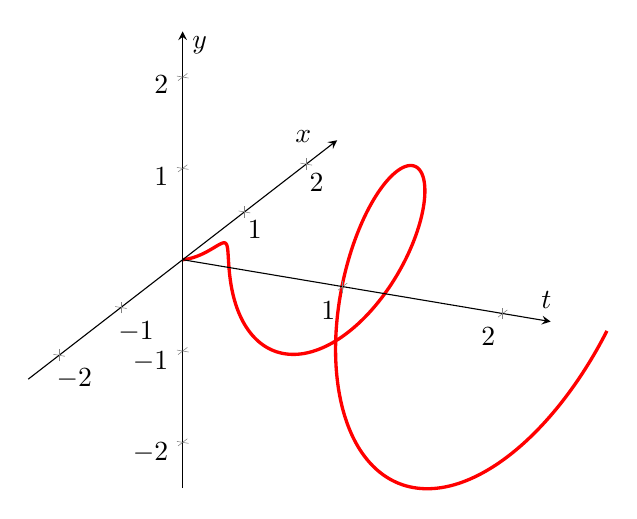
\begin{tikzpicture}[scale=1]\pgfplotsset{compat=1.8}
			\begin{axis}[enlargelimits=true,axis lines=center, axis on top, xlabel={$t$}, ylabel={$x$}, zlabel={$y$}, %axis equal,view={35}{340},,
				ymin=-2.5,ymax=2.5,zmin=-2.5,zmax=2.5,xmin=-0,xmax=2.3,	y post scale=1.8,z post scale=1.8]
				\addplot3[samples=500, very thick,red, domain = 0:2, samples y =0] ({x},{x*cos(6*deg(x))},{ x*sin(6*deg(x))});
			\end{axis}
		\end{tikzpicture}
	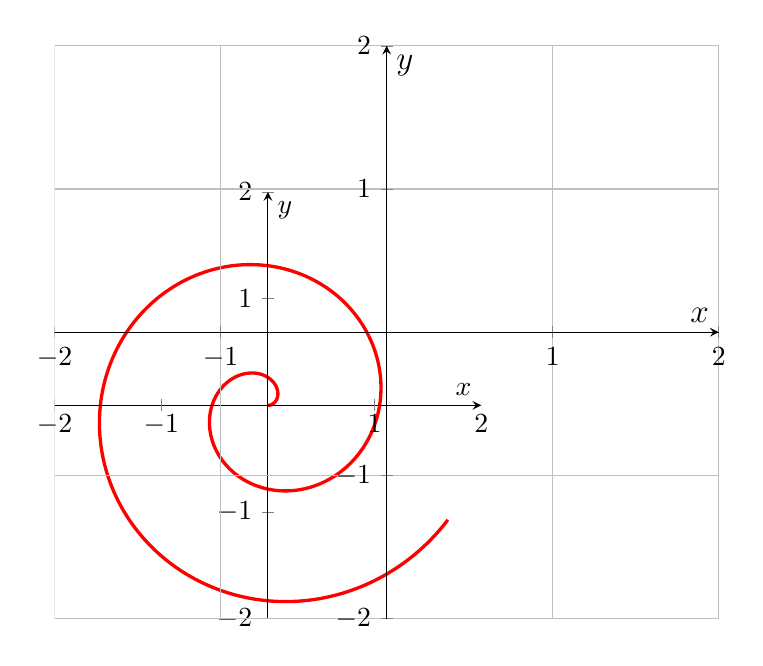
\begin{tikzpicture}\pgfplotsset{compat=1.8}
				\sld{\begin{axis}[height=7cm,width=7cm,enlargelimits=true,grid=major,  axis lines=center, axis on top, xlabel={$x$}, ylabel={$x$}, zlabel={$y$}, axis equal,view={90}{0},,
				ymin=-2,ymax=2,zmin=-2,zmax=2,xmin=0,xmax=2]
				\addplot3[grid=both,samples=500, very thick,red, domain = 0:2, samples y =0] ({x},{x*cos(6*deg(x))},{ x*sin(6*deg(x))});
			\end{axis}}
				\pl{\begin{axis}[ scale only axis, grid=major, axis lines=middle, inner axis line style={=>}, xlabel={\large $x$}, ylabel={\large $y$}, ytick={-2,-1,...,2}, xtick={-2,-1,...,2}, ymin=-2, ymax=2, xmin=-2, xmax=2, samples=50 ]
\addplot[color=black,thin] {0};

			\end{axis}}
		\end{tikzpicture}
	\end{center}
\end{exemple}


\bigskip

\sld{\vfill\pagebreak[5]}%%%%%%%%%%%%%%%

On peut munir $\mathcal F(I,E)$ de l'addition $\mathcal F(I,E) \times \mathcal F(I,E) \to \mathcal F(I,E)$ définie par  $(f,g) \mapsto f+g$  avec
\[
	(f+g)(t) = f(t)+g(t), \qquad \text{ pour tout $t\in I$.}
\]
Cette opération est associative, commutative, admet un élément neutre (la fonction nulle $t\mapsto 0$) et chaque $f\in \mathcal F(I,E)$ admet un opposé $-f$ définit par $(-f)(t)= -f(t)$. De plus pour tout $\alpha\in\R$ l'application $(\alpha,f) \mapsto \alpha f$ est une application $\R\times \mathcal F(I,E) \to \mathcal F(I,E)$ (appelée multiplication externe). On a 
\[
	(\alpha f) (t) = \alpha f(t), \qquad \text{ pour tout $t\in I$.}
\]
On a le résultat suivant:
\begin{proposition}\label{prop.revFIE}
	L'espace $\mathcal F(I,E)$ est un \rev{} (de dimension infinie). 
\end{proposition}

\begin{proof}
    La démonstration ne pose pas de problème particulier: il faut vérifier un à un les axiomes des \rev. Noter que c'est le fait que l'espace d'arrivée $E$ soit un \rev{} qui fait fonctionner le tout.
\end{proof}


\subsection{Limite et continuité}

%On note $(E,\snorm{\cdot})$ un \rev de dimension finie et $ $ une base de $E$.
On note toujours $E=\R^n$ muni de la base canonique et de la norme euclidienne. Soit $I$ un intervalle ouvert de $\R$ et $f:I\to E$ alors on note $f_i: I \to \R$ les fonctions coordonnées pour $i=1,\cdots,n$. Avec ces notations on a:
\begin{definition}[(limite)]
	On dit que $f$ admet une limite $\ell = \begin{psmallmatrix}\ell_1\\\vdots\\\ell_n\end{psmallmatrix}\in E$ quand $t$ tend vers $a\in I$ si $\lim_{t\to a}\limits  f_i(t) = \ell_i$ pour tout $i=1,\cdots,n$. Dans ce cas on a
	\[
		\lim_{t\to a} f(t) = \begin{pmatrix}\lim_{t\to a}\limits f_1(t) \\ \vdots \\ \lim_{t\to a}\limits f_n(t)\end{pmatrix} = \begin{pmatrix}\ell_1\\ \vdots \\ \ell_n\end{pmatrix} = \ell
	\]
\end{definition}
En bref, $f$ admet une limite en $a$ si toutes ses fonctions coordonnées convergent en $a$. Cette définition équivaut à $\lim_{t\to a} \limits \| f(t) - \ell\| =0 $ et on peut se ramener à la limite d'une fonction réelle. Si la limite existe, elle est unique.

\pl{\rep{4cm}}


\begin{remark}
	Cette définition s'adapte sans difficultés aux notions de limites à droite (\ie quand $t\to a$ avec $t>a$) noté $\lim_{t\to a^+} \limits f(t) $ ou $f(a^+)$ et limite à gauche  (\ie quand $t\to a$ avec $t<a$) notée $\lim_{t\to a^-}\limits  f (t)$ ou $f(a^-)$. Ainsi, si $f(a^+) = f(a^-) = \ell$ alors $f$ admet $\ell$ pour limite en $a$. 
\end{remark}

De même que dans le cas des fonctions réelles on a la caractérisation suivante:

\begin{proposition}[(caractérisation séquentielle)]
    Pour que $f$ admette une limite $\ell \in E$ en $a\in I$ il faut et il suffit que pour toute suite $(u_n)_{n\in\N}$ de $I$ telle que $\lim_n u_n = a \in I$ on ait $\lim_n f(u_n)= \ell \in E$ (ou autrement dit que pour tout $i=1,\cdots,n$ on a $f_i(u_n) \to \ell_i$ quand $n\to+\infty$). 
\end{proposition}

\sld{\vfill\pagebreak[5]}%%%%%%%%%%%%%%%
On rappelle que la continuité est une notion \emph{locale}. Plus précisément on a:
\begin{definition} 
	Soit $f:I\to E$ une fonction vectorielle. On dit que $f$ est \emph{continue} en $a\in I$ si 
\[ \redspace
	\lim_{t\to a }f(t)= f(a)
\]
En d'autre termes, $f$ est continue en $a\in I$  si
\[ \redspace
	\lim_{t\to a} \snorm{f(t) - f(a)} = 0
\]
\end{definition}
	Ainsi, une fonction vectorielle est dite continue en $a$ si toutes ses fonctions coordonnées sont continues en $a$. Si l'intervalle $I$ est minoré (resp. majoré), on peut étendre facilement la définition de continuité à droite (resp. à gauche) pour le réel $a$ situé à l'extrémité inférieure (resp. supérieure) de $I$.	
	
Une fonction est continue sur un intervalle $I$ si et seulement si elle est continue en tout point de $I$. Dans la suite, on notera $\mathcal C^0(I,E)$ l'ensemble des fonctions continues de $I\subset \R$ dans $E$.
	\begin{proposition}
		L'espace fonctionnel $\mathcal C^0(I,E)$ est un \rev.
	\end{proposition}

	\begin{proof}
	Même remarque que pour la preuve de la Proposition \ref{prop.revFIE}	
	\end{proof}

\sld{\vfill\pagebreak[5]}%%%%%%%%%%%%%%%
	\begin{definition}
		On dit que $f:I\to E$ est \emph{uniformément continue} sur $I$ si, pour tout $\varepsilon>0$, il existe $\delta>0$ tel que, pour tout $t,t'\in I$ on a 
		\[
			\abs{t-t'} <\delta \Rightarrow \snorm{f(t) - f(t')} < \varepsilon.
		\]
	\end{definition}

	\begin{proposition}[(Théorème de Heine)]
		Soit $I$ un intervalle fermé et borné de $\R$ et $E=\R^n$. Toute application continue de $I$ dans $E$ est uniformément continue sur $I$.
	\end{proposition}

\sld{\vfill\pagebreak[5]}%%%%%%%%%%%%%%%
\subsection{Dérivabilité}

Soit $E=\R^n$ muni de la base canonique et de la norme euclidienne. Soit $I$ un intervalle ouvert de $\R$ et $f:I\to E$ alors on note $f_i: I \to \R$ les fonctions coordonnées pour $i=1,\cdots,n$. Avec ces notations on a:
\begin{definition}[(dérivabilité)] 
	Soit $f:I\to E$ une fonction vectorielle. On dit que $f$ est dérivable en $a\in I$ si toutes les fonctions coordonnées de $f$ sont dérivables en $a$. On note
\[
	f'(a)= \begin{pmatrix}f_1'(a) \\ \vdots \\ f_n'(a)\end{pmatrix}
\]
\end{definition}
La dérivabilité est comme la continuité une définition locale. Une fonction vectorielle $f$ est dite dérivable sur $I$ si elle est dérivable en tout point de $I$.
%On dit que $f$ est différentiable en $a \in I$ s'il existe une fonction $h \mapsto \varepsilon(h)$ de $I$ dans $E$ et un vecteur $\ell \in E$ vérifiant,
%\[
%	f(a+h) -f(a) = h \ell + h\varphi(h)
%\]

\sld{\vfill\pagebreak[5]}%%%%%%%%%%%%%%%

Bien sûr, si les fonctions coordonnées sont suffisamment régulières, on peut généraliser la définition aux dérivées d'ordres supérieurs. On alors $f'' = \begin{psmallmatrix}
	f''_1\\ \vdots\\ f''_n
\end{psmallmatrix}$ et plus généralement on note $f^{(k)}= \begin{psmallmatrix}
	f^{(k)}_1\\ \vdots\\ f^{(k)}_n
\end{psmallmatrix}$ le vecteurs des dérivées $k$-ème. On notera enfin $\mathcal C^k(I, E)$ l'ensemble des fonctions vectorielles admettant une dérivée d'ordre $k$ continue (\ie dont les fonctions coordonnées sont $\mathcal C^k(I,\R)$).


\sld{\vfill\pagebreak[5]}%%%%%%%%%%%%%%%

On rappelle que le théorème des accroissements finis (TAF) pour une fonction $f:[a,b] \to \R$. Si $f$ est continue sur $[a,b]$ et dérivable sur $]a,b[$ alors il existe $c \in]a,b[$ tel que 
	\[f(b) - f(a) =  f'(c) (b-a) \]
Sous cette forme, le théorème ne se généralise pas aux fonctions vectorielles.
\begin{exemple}
 On considère la fonction vectorielle $t\mapsto (\sin(t) , \sin(2t))$.	
 \pl{\rep{4cm}}
\end{exemple}

\sld{\vfill\pagebreak[5]}%%%%%%%%%%%%%%%

On a le résultat plus faible suivant mais qui est valable pour les fonctions vectorielles et numériques:
\begin{theorem}[(Inégalité des accroissements finis)]
	Soit $f:[a,b] \to E$ une fonction vectorielle continue sur $[a,b]$ et dérivable sur $]a,b[$. %On suppose qu'il existe $\varphi:[a,b] \to \R$ continue sur $[a,b]$, dérivable sur $]a,b[$ et telle qu'en tout point $x$ de $]a,b[$ on ait l'inégalité
		%\[
	%		\snorm{f'(x)} \leq \varphi'(x)
	%	\]
	%	Alors, on a aussi la majoration suivante:
	%	\[
	%		\snorm{f(a) - f(b)} \leq \varphi(b) - \varphi(a)
	%	\]
	On suppose qu'il existe $M\geq 0$ tel que 
	\[
		\snorm{f'(x)} \leq M.
	\]
pour tout $x\in ]a,b[$. ALors 
	\[
		\snorm{f(a) -f(b) } \leq M (b-a).
	\]
		\label{TAF}
\end{theorem}


\sld{\vfill\pagebreak[5]}%%%%%%%%%%%%%%%

\section{Courbes paramétrées}

\subsection{Définitions}

Soit $E$ un \rev{}.

\begin{definition}
	On appelle \emph{courbe paramétrée} (on dit aussi \emph{arc paramétrée}) de $E$, un couple $\Gamma = (I,\phi)$ formé d'un intervalle de $I$ de $\R$ et d'une application $\phi:I \to E$ de classe $\Cc^1$ sur $I$. L'image $\phi(I) \subset E$ de $\phi$ est le \emph{support} de la courbe paramétrée $\Gamma$. 
\end{definition}

\pl{\rep{3cm}}

Lorsque $\phi$ est de classe $\Cc^k$ on dit que la courbe paramétrée est de classe $\Cc^k$.

\begin{exemple}
	\sld{	
\begin{enumerate}
\item Soit $E =\R^3$, un point $A\in E$ et $v\in E$ alors $\phi: t \mapsto A + tv$ pour tout $t\in\R$ est une droite affine passant par $A$ et de direction $v$.

\item Soit $I=[0,2\pi]$, $E=\R^2$ et $a,b>0$. Alors $\phi: t \mapsto (a\cos(t),b\sin(t))$ est une ellipse.
\end{enumerate}
}

\pl{\rep{3cm}}
\end{exemple}

\sld{\vfill\pagebreak[5]}%%%%%%%%%%%%%%%

\begin{exemple}
	$E =\R^3$ et $\phi: t \mapsto \left( \cos t, \sin t , \sinh t \right) \frac{1}{\cosh t} $ pour tout $t\in\R$.
	\begin{center}
		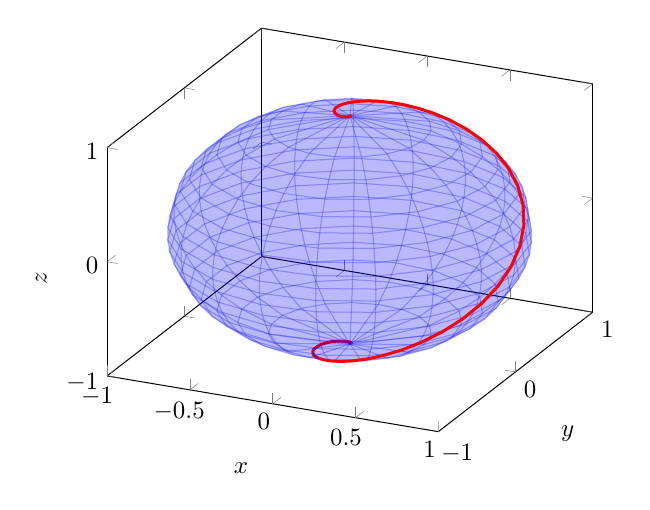
\begin{tikzpicture}[scale=.9]
			\begin{axis}[xlabel = $x$,ylabel=$y$,zlabel=$z$,, xmin=-1,xmax=1,ymin=-1,ymax=1,zmin=-1,zmax=1]
				\addplot3[, axis equal,samples=100,red, very thick, domain = -5:-pi/2, samples y =0] ({cos(deg(x))/cosh(x)},{sin(deg(x))/cosh(x)},{tanh(x)});
				\addplot3[surf,shader=flat,opacity=.15,z buffer=sort,blue,samples=20,domain=-1:1,y domain=0:2*pi]
({sqrt(1-x^2) * cos(deg(y))},
{sqrt( 1-x^2 ) * sin(deg(y))},
x);
				\addplot3[ axis equal,samples=100,red, very thick, domain = -pi/2:10, samples y =0] ({cos(deg(x))/cosh(x)},{sin(deg(x))/cosh(x)},{tanh(x)});
			\end{axis}
		\end{tikzpicture}
	\end{center}
	Pour des détails concernant la fonction $t\mapsto \cosh t$ on pourra voir \url{http://exo7.emath.fr/cours/ch_chainette.pdf}. Concernant les fonctions de la trigonométrie hyperbolique voir \cite{tt1} ou \cite{exo7} Chapitre 10.
\pl{\rep{10cm}}
\end{exemple}

\sld{\vfill\pagebreak[5]}%%%%%%%%%%%%%%%

\begin{exemple} Le trèfle gauche: $t\mapsto\begin{pmatrix}
			\cos(t) + 2\cos(2t) \\
			\sin(t) - 2\sin(2t)\\
			-2\sin(3t)
		\end{pmatrix}$
	
	\begin{center}
		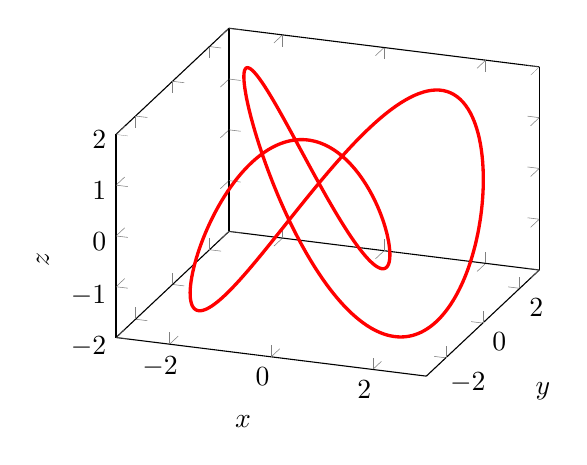
\begin{tikzpicture}
			\begin{axis}[height=6cm,xlabel = $x$,ylabel=$y$,zlabel=$z$,view={20}{20},  axis equal,xmin=-3,xmax=3,ymin=-3,ymax=3,zmin=-2,zmax=2]
				\addplot3[samples=500, very thick,red, domain = -0:10, samples y =0] ({cos(deg(x)) + 2*cos(deg(2*x))},{sin(deg(x)) - 2* sin(deg(2*x))},{-2*sin(deg(3*x))});
			\end{axis}
\end{tikzpicture}
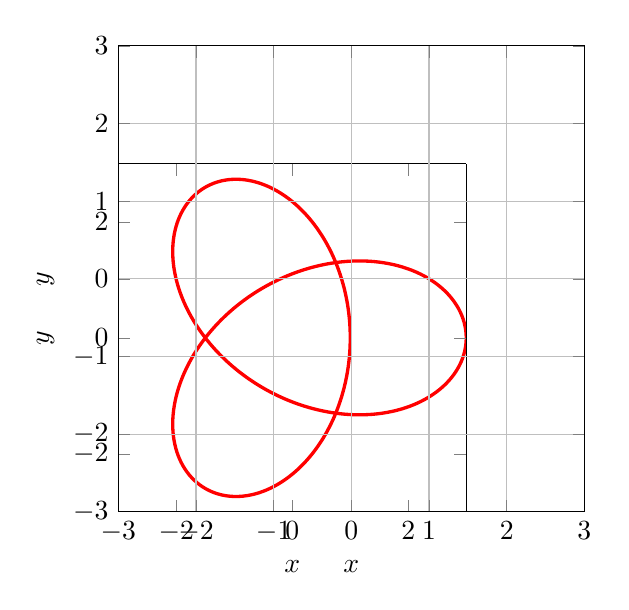
\begin{tikzpicture}%
	\sld{\begin{axis}[height=6cm,width=6cm, xlabel = $x$,ylabel=$y$,view={0}{90}, xmin=-3,xmax=3,ymin=-3,ymax=3,zmin=-3,zmax=3]
			\addplot3[samples=500, very thick,red, domain = -0:10, samples y =0] ({cos(deg(x)) + 2*cos(deg(2*x))},{sin(deg(x)) - 2* sin(deg(2*x))},{-2*sin(deg(3*x))});
			\end{axis}}%
	\pl{\begin{axis}[height=7.5cm,width=7.5cm, grid=major, inner axis line style={=>}, xlabel={$x$}, ylabel={$y$}, ytick={-3,-2,...,3}, xtick={-3,-2,...,3}, ymin=-3, ymax=3, xmin=-3, xmax=3, samples=5 ]\addplot[color=gray,thin] {10};
			\end{axis}}
\end{tikzpicture}
	\end{center}
\end{exemple}
\begin{definition}
    Une courbe paramétrée continue $\Gamma =(I,\phi)$ est \emph{simple} si tout point $M = \phi \in \phi(I)$ a un unique antécédents par  $\phi$.
            \begin{center}
                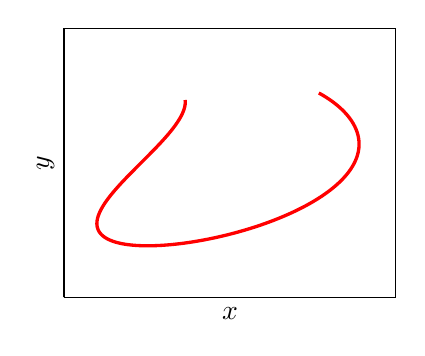
\begin{tikzpicture}
                    \begin{axis}[height=3cm,xlabel = $x$,ylabel=$y$,zlabel=$z$,height=5cm, axis equal,view={0}{90},, xmin=-2.5,xmax=1.5,ymin=-1,ymax=1,zmin=-0,zmax=0,xtick=\empty, ytick=\empty,]
                        \addplot3[samples=500, very thick,red, domain = -2:.5, samples y =0] ({cos(deg(3*x)) + x},{ sin(deg(2*x))},{0});
                    \end{axis}
                \end{tikzpicture}
            \end{center}\sld{\vfill\pagebreak[5]}%%%%%%%%%%%%%%%
            Un point \emph{multiple} est un point qui possède plusieurs antécédent par $\phi$.
    \begin{enumerate}
    %\item \emph{ $\boldsymbol{\Cc^1}$ par morceau} si $I=[a,b]$ et il existe une subdivision $a_0=a < a_1 < \cdots< b=a_m$ telle que la restriction $\Gamma_{a_i,a_{i+1}} = ([a_{i-1},a_{i}],\phi)$ est de classe $\Cc^1$ pour tout $i=\left\{ 0,\cdots,m-1 \right\}$.
        %\begin{center}
            %\begin{tikzpicture}
                %\begin{axis}[height=3cm,xlabel = $x$,ylabel=$y$,zlabel=$z$, height=5cm,axis equal,view={0}{90},, xmin=-2,xmax=3,ymin=-3,ymax=3,zmin=-0,zmax=0,xtick=\empty, ytick=\empty,]
                %\addplot3[samples=500, very thick,red, domain = -0:pi*3/2, samples y =0] ({cos(deg(2*x)) + 2*cos(deg(x))},{2*sin(deg(x)) - sin(deg(2*x))},{0});
            %\end{axis}
        %\end{tikzpicture}
        %\end{center}\sld{\vfill\pagebreak[5]}%%%%%%%%%%%%%%%
       % \item 
            %\item \emph{fermé} si $I=[a,b]$,  $\Gamma$ est simple (sur l'inétérieur d'une période) et $\phi(a) = \phi(b)$.
    %\begin{center}
            %\begin{tikzpicture}
            %\begin{axis}[height=3cm,xlabel = $x$,ylabel=$y$,zlabel=$z$,height=5cm, axis equal,view={0}{90},, xmin=-2,xmax=2,ymin=-2,ymax=2,zmin=-0,zmax=0,xtick=\empty, ytick=\empty,]
                %\addplot3[samples=500, very thick,red, domain = -pi:pi, samples y =0] ({cos(deg(x)) *(1+ 0.3*sin(deg(12*x))) },{ sin(deg(x)) *(1+ 0.3*sin(deg(12*x)))},{0});
            %\end{axis}
        %\end{tikzpicture}
        %\end{center}
    \end{enumerate}
\end{definition}

\sld{\vfill\pagebreak[5]}%%%%%%%%%%%%%%%


\subsection{Interprétation cinématique} 

Soit $(I,\phi)$ une courbe paramétrée. Si $t\in I$ désigne le temps:
\begin{enumerate}
	\item $\phi(t) \in E$ est la position d'un mobile ponctuel à l'instant $t\in I$. 
	\item  $\phi'(t)$ est la vitesse du mobile.
	\item $\phi''(t)$ est l'accélération du mobile. 
	\item le support de $\Gamma$ correspond à la trajectoire du mobile.
\end{enumerate}

\pl{\rep{5cm}}


Le chemin parcouru par le mobile ne change pas si on modifie sa vitesse instantanée.  Pour formaliser cela on introduit la définition suivante:

\begin{definition}
	Soient $I$ et $J$ deux intervalles ouverts de $\R$ et $\theta: I \to J$ une fonction bijective (on note $\theta^{-1}$ son inverse). Si $k\in\N^*$, on dit que $\theta$  est un $\Cc^k$ difféomorphisme si $\theta$ est  de classe $\Cc^k(I,J)$ \emph{et} $\theta^{-1}$ est de classe $\Cc^k(J,I)$.
\end{definition}
\begin{remark}
    La définition d'un difféomorphisme $\theta$ implique que les dérivées $\theta'$ et $(\theta^{-1})' = \frac{1}{\theta' \circ \theta^{-1}}$ ne s'annulent pas sur leur intervalle de définition respectif. 
\end{remark}

\begin{exemple}
	L'application $\theta: t \mapsto t^3$ n'est pas un $\Cc^1$ difféomorphisme de $\R$ dans $\R$. Mais l'application $t\mapsto t^3 +t$ est un $\Cc^1$ difféomorphisme de $\R$ dans $\R$.
	\pl{\rep{7cm}}
\end{exemple}

\sld{\vfill\pagebreak[5]}%%%%%%%%%%%%%%%


Les $\Cc^k$ difféomorphismes sont les changements de variables ayant une régularité suffisante pour reparamétrer les courbes de classe $\Cc^k$ tout en conservant cette régularité. Plus précisément on a:
\begin{definition}
	[(Paramétrage admissible)]
	Soit $\Gamma_0 = (I,\phi)$ une courbe paramétrée de classe $\Cc^k$ ($k\geq 1$) et $J$ un intervalle de $\R$. On dit que $\theta: J \to I$ est un changement de paramètre admissible si c'est un $ \Cc^k$-difféomorphisme de $J$ sur $I$. On dit que $\Gamma_1 = (J,\phi \circ \theta)$ est un autre \emph{paramétrage admissible} de $\Gamma_0$.
\end{definition}
	\pl{\rep{4cm}}

\begin{remark}
Les arcs paramétrés $\Gamma_0$ et $\Gamma_1$ ont le même support. C'est la vitesse de parcours qui change.
\end{remark}

\sld{\vfill\pagebreak[5]}%%%%%%%%%%%%%%%


\begin{exemple} Voici le graphe de $\Gamma_0=(\R, \phi)$ où $\phi: t \mapsto (\cos(8t),\sin(8t))$:
	\begin{center}	
            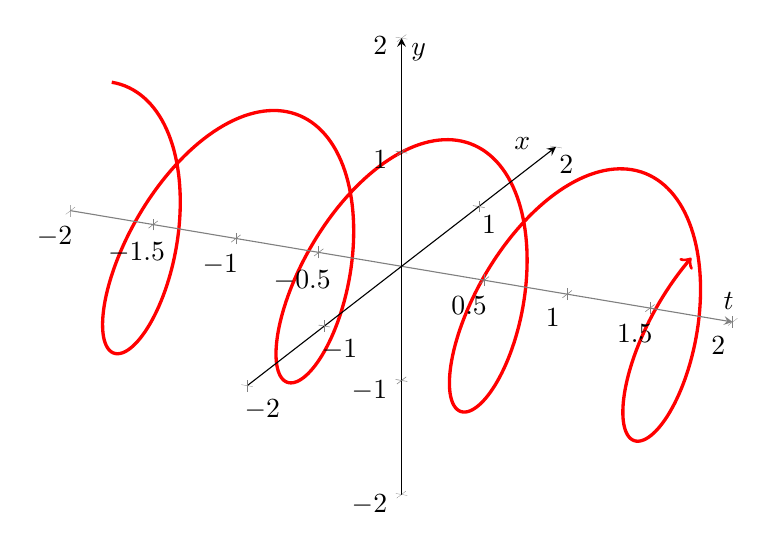
\begin{tikzpicture}[scale=1]\pgfplotsset{compat=1.8}
                \begin{axis}[enlargelimits=true,axis lines=center, axis on top, xlabel={$t$}, ylabel={$x$}, zlabel={$y$}, x axis line style=gray, %axis equal,view={35}{340},,
                    ymin=-2,ymax=2,zmin=-2,zmax=2,xmin=-2,xmax=2, x post scale=1.8, y post scale=1.8,z post scale=1.8]
                    \addplot3[samples=500, very thick,red, domain = -2:2, samples y =0,->] ({x},{sin(6*deg(x))},{cos(6*deg(x))});
                \end{axis}
            \end{tikzpicture}
		\begin{tikzpicture}[scale=1]\pgfplotsset{compat=1.8}
			\begin{axis}[enlargelimits=true,axis lines=center, axis on top, xlabel={$t$}, ylabel={$x$}, zlabel={$y$}, axis equal,view={90}{0},
                            ymin=-2,ymax=2,zmin=-2,zmax=2,xmin=-2,xmax=2,]
                            \addplot3[samples=500, very thick,red, domain = -2:2, samples y =0,->] ({x},{sin(6*deg(x))},{cos(6*deg(x))});
			\end{axis}
		\end{tikzpicture}
	\end{center}
\sld{\vfill\pagebreak[5]}%%%%%%%%%%%%%%%
Traçons maintenant le graphe de $\Gamma_1=(\R, \phi_2 )$ où $\phi_2: t \mapsto ( \cos( (3t/2)^{3} + 3t/2 ),\sin( (3t/2)^{3} +3t/2 ))$:
		\begin{center}	
			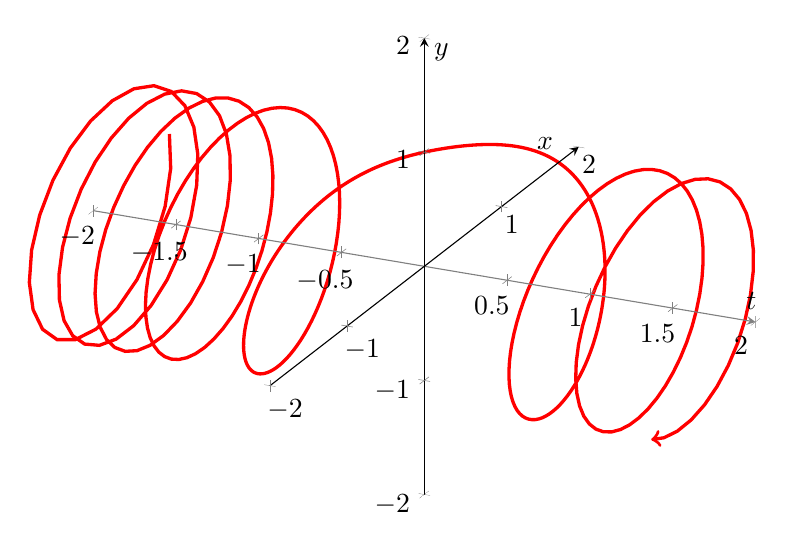
\begin{tikzpicture}[scale=1]\pgfplotsset{compat=1.8}
				\begin{axis}[enlargelimits=true,axis lines=center, axis on top, xlabel={$t$}, ylabel={$x$}, zlabel={$y$}, x axis line style=gray,%axis equal,view={35}{340},,
                                    ymin=-2,ymax=2,zmin=-2,zmax=2,xmin=-2,xmax=2,x post scale=1.8,y post scale=1.8,z post scale=1.8]
                                %\addplot3[samples=500, very thick,red, domain = -10.4:10.4, samples y =0] ({x*x*x/(8*8*8)},{sin(deg(x))},{cos(deg(x))});
                                \addplot3[samples=500, very thick,red, domain = -2:1.6, samples y =0,->] ({x},{sin(deg( (1.5*x)^3 +(1.5*x)) )},{cos( deg(((1.5*x)^3 + (1.5*x)) ))});
				\end{axis}
			\end{tikzpicture}
			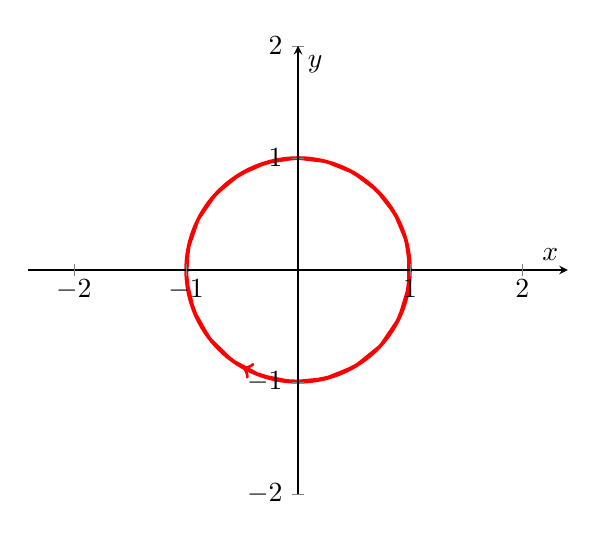
\begin{tikzpicture}[scale=1]\pgfplotsset{compat=1.8}
				\begin{axis}[enlargelimits=true,axis lines=center, axis on top, xlabel={$t$}, ylabel={$x$}, zlabel={$y$}, axis equal,view={90}{0},,
                                    ymin=-2,ymax=2,zmin=-2,zmax=2,xmin=-2,xmax=2]
                                \addplot3[samples=500, very thick,red, domain = -2:1.6, samples y =0,->] ({x},{sin(deg( (1.5*x)^3 +(1.5*x)) )},{cos( deg(((1.5*x)^3 + (1.5*x)) ))});
				\end{axis}
			\end{tikzpicture}
		\end{center}
		Les deux courbes $\Gamma_0$ et $\Gamma_1$ ont le même support et décrivent toutes deux le cercle unité du plan. Mais les vitesses de parcours sont différentes.
\end{exemple}

\begin{definition}
On dit qu'une courbe paramétrée $\Gamma=(I,\phi )$ de classe $\mathcal C^1$ est \emph{régulière} si pour tout $t\in I$ $\phi'(t) \neq 0$.
\end{definition}

\begin{remark}
Si $\Gamma_0 = (I,\phi)$ est une courbe paramétrée régulière et $\Gamma_1 = (J, \varphi =\phi \circ \theta)$ est une reparamétrisation admissible de $\Gamma_0$ alors $\Gamma_1$ est aussi régulière. En effet, comme $\theta: J \to I$ est une $\mathcal C^1$-difféomorphisme, on a:
            \[
                \forall t \in J, \varphi' (t) = \phi'(\theta(t)) \theta'(t) \neq 0.
            \]
\end{remark}

\begin{exemple}
    Considérons la courbe paramétrée définie par $\phi(t) = (t,t^2)$ pour $t\in\R$:
    %Une courbe paramétrée régulière admet une tangente en tout point (voir plus bas). La réciproque n'est pas vraie. 
            \begin{center}
                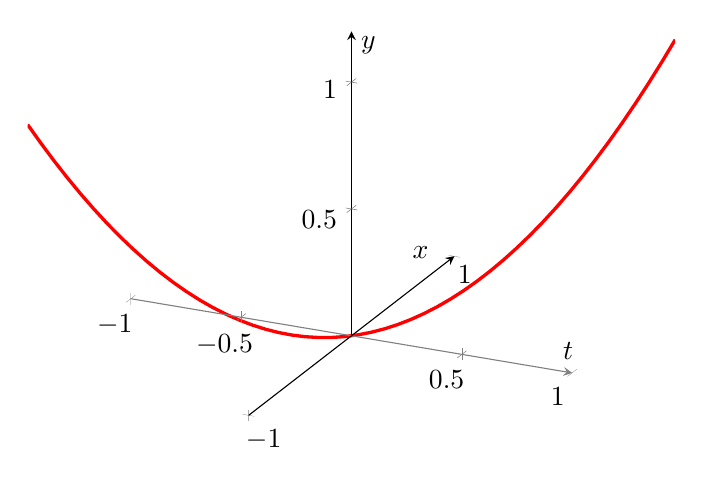
\begin{tikzpicture}[scale=1]\pgfplotsset{compat=1.8}
                    \begin{axis}[enlargelimits=true,axis lines=center, axis on top, xlabel={$t$}, ylabel={$x$}, zlabel={$y$}, x axis line style=gray, ymin=-1,ymax=1,zmin=0,zmax=1.2,xmin=-1,xmax=1,x post scale=1.2,y post scale=1.2,z post scale=1.2]
                    \addplot3[samples=50, very thick,red, domain =-1:1, samples y =0] ({x},{x},{x^2});
                    \end{axis}
                \end{tikzpicture}\hfill%
                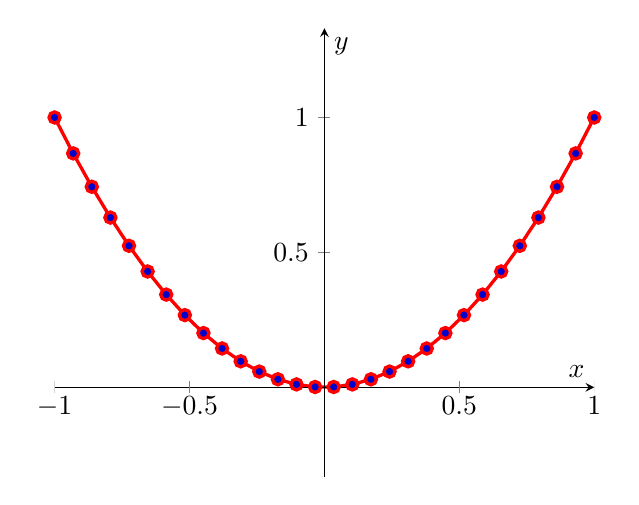
\begin{tikzpicture}[scale=1]\pgfplotsset{compat=1.8}
			\begin{axis}[enlargelimits=false,axis lines=center, axis on top, xlabel={$t$}, ylabel={$x$}, zlabel={$y$}, axis equal,view={90}{0},
                    ymin=-1,ymax=1,zmin=0,zmax=1,xmin=-.1,xmax=.1,%x post scale=1.8,y post scale=1.8,z post scale=1.8
                    ]
                        \addplot3+[samples=30, very thick,red, domain = -1:1, samples y =0] ({0},{x},{x^2});
			\end{axis}
		\end{tikzpicture}
            \end{center}
            La courbe paramétrée $\Gamma_1$ définie par $\phi_1(t)=(t^3 +t, (t^3 +t )^2)$ avec $t\in \R$ est une reparamétrisation admissible de $\Gamma$: 
            \begin{center}
                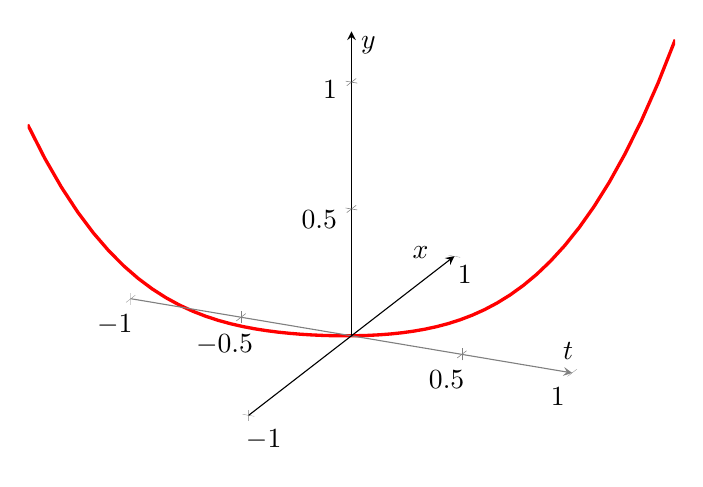
\begin{tikzpicture}[scale=1]\pgfplotsset{compat=1.8}
                    \begin{axis}[enlargelimits=true,axis lines=center, axis on top, xlabel={$t$}, ylabel={$x$}, zlabel={$y$}, x axis line style=gray, ymin=-1,ymax=1,zmin=0,zmax=1.2,xmin=-1,xmax=1,x post scale=1.2,y post scale=1.2,z post scale=1.2]
                        %\addplot3[samples=500, very thick,red, domain =-pi/4:pi/4, samples y =0] ({x},{tan(deg(x))},{(tan(deg(x)))^2});
                    \addplot3[samples=50, very thick,red, domain =-1:1, samples y =0] ({x},{(x^3 + x) /2},{((x^3 + x) /2)^2});
                    \end{axis}
                \end{tikzpicture}\hfill%
                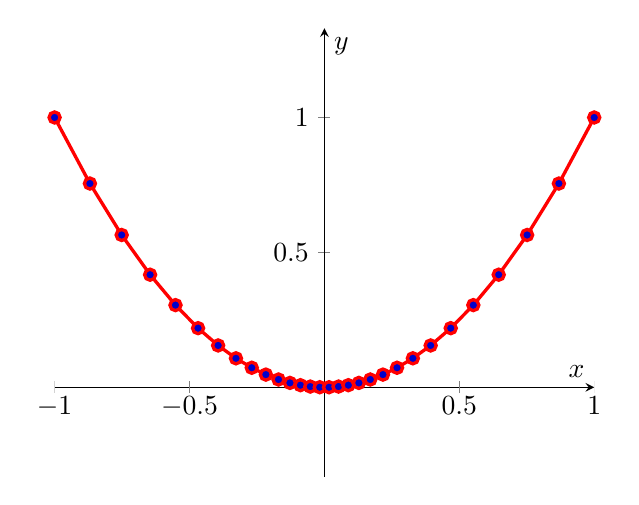
\begin{tikzpicture}[scale=1]\pgfplotsset{compat=1.8}
			\begin{axis}[enlargelimits=false,axis lines=center, axis on top, xlabel={$t$}, ylabel={$x$}, zlabel={$y$}, axis equal,view={90}{0},
                    ymin=-1,ymax=1,zmin=0,zmax=1,xmin=-.1,xmax=.1,%x post scale=1.8,y post scale=1.8,z post scale=1.8
                    ]
                        \addplot3+[samples=30, very thick,red, domain =-1:1, samples y =0] ({0},{(x^3 + x) /2},{((x^3 + x) /2)^2});
			\end{axis}
		\end{tikzpicture}
            \end{center}
    
La courbe paramétrée $\Gamma_2$ définie par $\phi_2(t)=(t^3,t^6)$ avec $t\in \R$ n'est pas une reparamétrisation admissible de $\Gamma$: 
            \begin{center}
                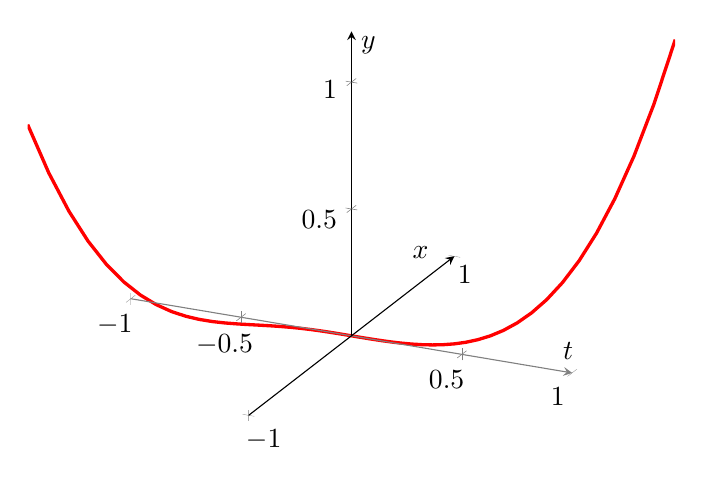
\begin{tikzpicture}[scale=1]\pgfplotsset{compat=1.8}
                    \begin{axis}[enlargelimits=true,axis lines=center, axis on top, xlabel={$t$}, ylabel={$x$}, zlabel={$y$}, x axis line style=gray, ymin=-1,ymax=1,zmin=0,zmax=1.2,xmin=-1,xmax=1,x post scale=1.2,y post scale=1.2,z post scale=1.2]
                    \addplot3[samples=50, very thick,red, domain =-1:1, samples y =0] ({x},{x^3},{x^6});
                    \end{axis}
                \end{tikzpicture}\hfill%
                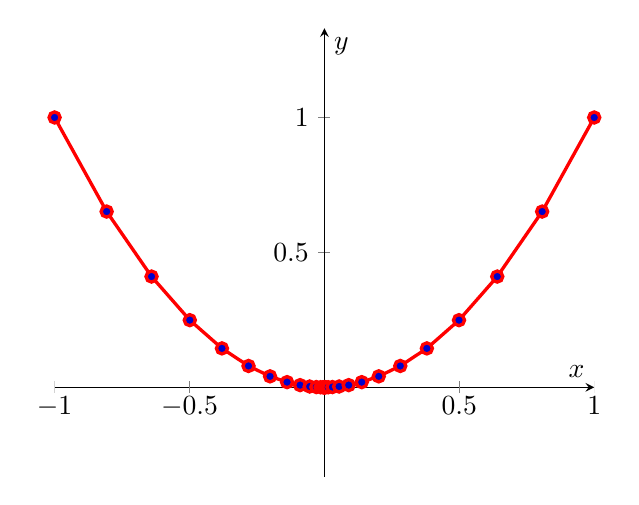
\begin{tikzpicture}[scale=1]\pgfplotsset{compat=1.8}
			\begin{axis}[enlargelimits=false,axis lines=center, axis on top, xlabel={$t$}, ylabel={$x$}, zlabel={$y$}, axis equal,view={90}{0},
                    ymin=-1,ymax=1,zmin=0,zmax=1,xmin=-.1,xmax=.1,%x post scale=1.8,y post scale=1.8,z post scale=1.8
                    ]
                        \addplot3+[samples=30, very thick,red, domain = -1:1, samples y =0] ({0},{x^3},{x^6});
			\end{axis}
		\end{tikzpicture}
            \end{center}
            La courbe géométrique associée est toujours la parabole d'équation $y=x^2$ mais on a ``créé un arrêt'' car $ \phi_3'(0)$ est nul. 
    \end{exemple}

\sld{\vfill\pagebreak[5]}%%%%%%%%%%%%%%%
\section{\'Etude locale d'un arc}

Soit $\Gamma=(I,\phi)$ une courbe paramétrée de classe $\Cc^k$, $k\in\N^*$ suffisamment grand. La formule de Taylor-Young en $t_0\in I$ s'écrit 
\[
	\phi(t_0 + h) =  \phi(t_0) + h \phi'(t_0) + \frac{h^2}{2} \phi''(t_0) + \cdots + \frac{h^k}{k!} \phi^{(k)}(t_0) + \sabs{h}^k \varepsilon(h). 
\]
où $\varepsilon: \R \to E$ satisfait $\lim_{h\to 0} \varepsilon(h) =0$. Si les vecteurs dérivées de $\phi$ ne sont pas tous nul en $t_0$, on note:  %existe $i\in \N^*$ tel que $\phi^{(i)}(t_0)\neq 0$, on note 

\begin{enumerate}
	\item $p$ le plus petit entier non nul tel que $\phi^{(p)}(t_0)\neq 0 $.
	\item  $q$ le premier entier supérieur à $p$ tel que $\phi^{(q)}(t_0)$ ne soit pas colinéaire à $\phi^{(p)}(t_0) $. Autrement dit, pour tout entier $i\in\left\{ p,\cdots,q-1\right\}$, il existe $\lambda_i\in\R$ tel que: $\phi^{(i)}(t_0) = \lambda_i \phi^{(p)} (t_0)$. 
\end{enumerate}\sld{\vfill\pagebreak[5]}%%%%%%%%%%%%%%%
La formule de Taylor-Young devient:
\[
	\phi(t_0 + h) =  \phi(t_0) + \left( \sum_{i=p}^{q-1} \lambda_i \frac{h^i}{i!} \right) \phi^{(p)}(t_0) + \frac{h^q}{q!} \phi^{(q)}(t_0)+ \sabs{h}^q \varepsilon(h).
\]
où $\varepsilon: \R \to E$ est tel que $\lim_{h\to 0} \varepsilon(h) =0$.

\begin{definition}
	Le point $\phi(t_0)$ est un point:
	\begin{enumerate}
		\item \emph{régulier} si $\phi'(t_0) \neq 0$ (cas $p=1$). 
		\item \emph{stationnaire} si $\phi'(t_0) =0$ (cas $p>1$). 
	\item \emph{birégulier} si $\phi'(t_0)$ et $ \phi''(t_0)$ ne sont pas colinéaires  ($p=1$ et  $q=2 $).
	\end{enumerate}
\end{definition}

\begin{definition}
	La \emph{tangente} à l'arc $\Gamma$ au point $M_0 = \phi(t_0)$ est la droite affine passant par $M_0$ et dirigée par le vecteur $\phi^{(p)}(t_0)$.
\end{definition}
 \pl{\rep{3cm}}

\begin{remark}
	L'entier $p$ et la droite tangente $\R\phi^{(p)}(t_0)$ sont invariant par changement de paramétrisation admissible.
\end{remark}

\begin{exemple}
	Retour sur $E =\R^3$ et $\phi: t \mapsto \left( \cos t, \sin t , \sinh t \right) \frac{1}{\cosh t} $ pour tout $t\in\R$. On montre que $\prs{\phi(t),\phi'(t)} = 0$ pour tout $t\in\R$.
	\pl{\rep{5cm}}
\end{exemple}
\sld{\vfill\pagebreak[5]}%%%%%%%%%%%%%%%
\begin{defprop}
	On se place dans le cas $E=\R^2$. On pose $M_0=\phi(t_0)$, les vecteurs $v = \phi^{(p)}(t_0) $ et $w = \phi^{(q)}(t_0)$  forment un base de $\R^2$ et $(M_0,v,w)$ est un repère du plan.
\begin{enumerate}
\item Cas $p$ impair et $q$ pair: point \emph{ordinaire}.
	\begin{center}
		\input{../chap_courbes/figures/fig_courbes_part3_06.tex}
	\end{center}
\item Cas $p$ impair et $q$ impair: point \emph{d'inflexion}.
	\begin{center}
		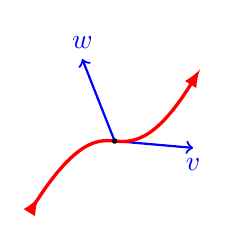
\begin{tikzpicture}[scale=1]

\begin{scope}[rotate=-5] 

  \draw[->,thick, blue] (0,0)--(1,0) node[below] {${v}$}; 
  \draw[->,thick, blue] (0,0)--(-0.5,1) node[above] {${w}$}; 
  \draw [>->,>=latex,very thick, color=red] (-1,-1) .. controls (-0.5,0) and (-0.2,0) .. (0,0) .. controls (0.2,0) and (0.5,0) .. (1,1);
 \fill (0,0) circle (1pt);
\end{scope}
\end{tikzpicture}

	\end{center}\sld{\vfill\pagebreak[5]}%%%%%%%%%%%%%%%
\item Cas $p$ pair et $q$ impair: point \emph{rebroussement de première espèce}.
	\begin{center}
		\input{../chap_courbes/figures/fig_courbes_part3_08.tex}
	\end{center}
\item Cas $p$ pair et $q$ pair: point \emph{rebroussement de deuxième espèce}.
	\begin{center}
		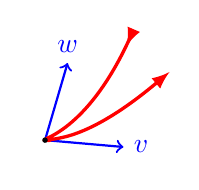
\begin{tikzpicture}[scale=1]

\begin{scope}[rotate=-5] 

  \draw[->, thick, blue] (0,0)--(1,0) node[right] {${v}$}; 
  \draw[->, thick, blue] (0,0)--(0.2,1) node[above] {${w}$}; 
  \draw [>->,>=latex,very thick, color=red] (1,1.5) .. controls (0.5,0) and (-0.2,0) .. (0.05,0.0) .. controls (0.1,0.05) and (0.5,0) .. (1.5,1);
 \fill (0,0) circle (1pt);
\end{scope}
\end{tikzpicture}

	\end{center}
\end{enumerate}
\end{defprop}

\pl{\rep{6cm}}
\sld{\vfill\pagebreak[5]}%%%%%%%%%%%%%%%

\section{\'Etude globale d'un arc paramétré - Cas plan ($E=\R^2$)}


\subsection{Branches infinies}

Soit $\Gamma=(I,\phi)$ un arc paramétré du plan $\R^2$ muni de la base canonique $(i,j)$. Pour $t\in I$, on pose $\phi(t) = (x(t),y(t))$ et $\snorm{\phi} = \sqrt{x^2(t) + y^2(t)}$. Dans ce qui suit, $a$ désigne une borne de $I$ (éventuellement infinie).

\begin{definition}
	On dit que $\Gamma$ admet une \emph{branche infinie} lorsque $t\to a$ si $\lim_{t\to a} \snorm{\phi(t)} = +\infty$
\end{definition}
\sld{\vfill\pagebreak[5]}%%%%%%%%%%%%%%%

Plusieurs cas se présentent 
\begin{enumerate}
	\item Si $\lim_{t\to a} \abs{x(t)} = +\infty$ et  $\lim_{t\to a} \abs{y(t)} = y_0$, alors la courbe $\Gamma$ admet la droite horizontale d'équation $y=y_0$ pour \emph{asymptote}.
		\begin{center}
			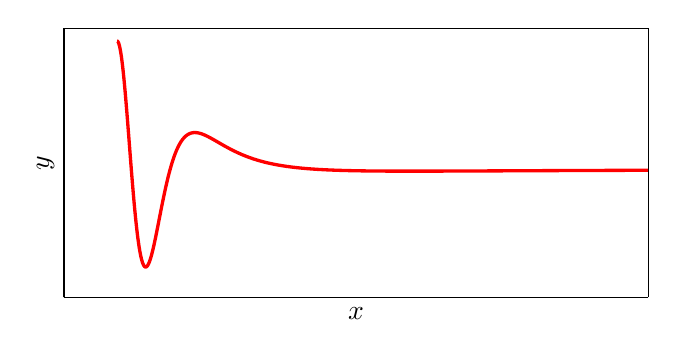
\begin{tikzpicture}
				\begin{axis}[xlabel = $x$,ylabel=$y$,zlabel=$z$,height=5cm,width=9cm,view={0}{90},, xmin=-1,xmax=10,ymin=-1,ymax=1.1,zmin=-0,zmax=0,xtick=\empty, ytick=\empty,]
					\addplot3[samples=500, very thick,red, domain = -0:pi/2, samples y =0] ({ tan(deg(x)) },{ (cos(deg(x)))^2 * cos(deg(6*x)) },{0});%CUBIQUE D'AGNESI
				\end{axis}
			\end{tikzpicture}
		\end{center}\sld{\vfill\pagebreak[5]}%%%%%%%%%%%%%%%

	\item Si $\lim_{t\to a} \abs{x(t)} = x_0$ et  $\lim_{t\to a} \abs{y(t)} = +\infty$, alors la courbe $\Gamma$ admet la droite verticale d'équation $x=x_0$ pour \emph{asymptote}.
		\begin{center}
			\begin{tikzpicture}
				\begin{axis}[xlabel = $x$,ylabel=$y$,zlabel=$z$,height=5cm,,view={0}{90},xmin=-2,xmax=4,ymin=-1,ymax=8,zmin=-0,zmax=0,xtick=\empty, ytick=\empty,
					]
					\addplot3[samples=500, very thick,red, domain = 0:10, samples y =0] ({ x^2 /(1+x^2) },{ x^3/(1+x^2)},{0});%CISSOÏDE DE DIOCLÈS
				\end{axis}
			\end{tikzpicture}
		\end{center}\sld{\vfill\pagebreak[5]}%%%%%%%%%%%%%%%

	\item On suppose que $\lim_{t\to a} \abs{x(t)} = +\infty$ et  $\lim_{t\to a} \abs{y(t)} = +\infty$, alors 
		\begin{enumerate}
			\item Si $\lim_{t\to a} \frac{y(t)}{x(t)} = 0$, on dit que $\Gamma$ admet une branche parabolique de direction $\R i$.
		\begin{center}
			\begin{tikzpicture}
				\begin{axis}[xlabel = $x$,ylabel=$y$,zlabel=$z$,height=6cm,width=10cm,view={0}{90},, xmin=-1,xmax=10,ymin=-1,ymax=5,zmin=-0,zmax=0,xtick=\empty, ytick=\empty,
					]
					\addplot3[samples=500, very thick,red, domain = -0:10, samples y =0] ({ (x+ 0*sin(deg(12*x)) )^2   },{ x+ ( x^2 /(1+x^2))*.6*sin(deg(6*x)) },{0});%CISSOÏDE DE DIOCLÈS
				\end{axis}
			\end{tikzpicture}
		\end{center}
			\item Si $\lim_{t\to a} \frac{y(t)}{x(t)} = \pm \infty$, on dit que $\Gamma$ admet une branche parabolique de direction $\R j$.\sld{\vfill\pagebreak[5]}%%%%%%%%%%%%%%%

			\item Si $\lim_{t\to a} \frac{y(t)}{x(t)} = \alpha$, deux cas se présentent
				\begin{enumerate}
					\item  Si $\lim_{t\to a} y(t) - \alpha x(t) =  \pm \infty$, on dit que $\Gamma$ admet une branche parabolique de direction $\R (i + \alpha j)$.
                                        \item  Si $\lim_{t\to a} y(t) - \alpha x(t) =  \beta$, on dit que $\Gamma$ admet la droite d'équation $y = \alpha x + \beta$ pour asymptote. Dans ce cas, on étudie la position de la courbe $\Gamma$ par rapport à l'asymptote. Pour cela, on étudie le signe de  $(y(t) - \alpha x(t) - \beta)$ au voisinage de $a$.
	\begin{center}
			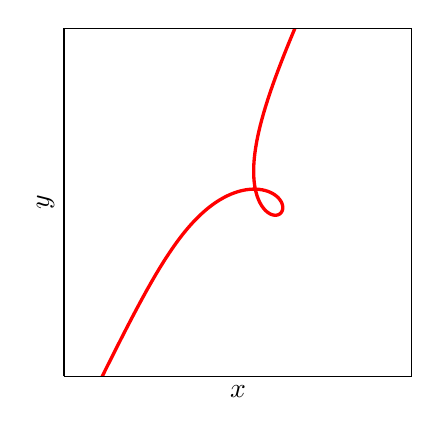
\begin{tikzpicture}
				\begin{axis}[xlabel = $x$,ylabel=$y$,zlabel=$z$,height=6cm,width=6cm,view={0}{90},, xmin=-8,xmax=8,ymin=-8,ymax=8,zmin=-0,zmax=0,xtick=\empty, ytick=\empty,
					]
					\addplot3[samples=500, very thick,red, domain = -10:10, samples y =0] ({2*(1-x^2)/(1+x^2) -x },{ 2*x * (1-x^2)/(1+x^2)  },{0});%CISSOÏDE DE DIOCLÈS
				\end{axis}
			\end{tikzpicture}
		\end{center}
				\end{enumerate}
		\end{enumerate}
\end{enumerate}

\sld{\vfill\pagebreak[5]}%%%%%%%%%%%%%%%

\section{Longueur et abscisse curviligne}

\begin{definition}
	Soit une courbe $\Gamma$ paramétrée par $\phi:[a,b] \to E$ de classe $\Cc^1$. La \emph{longueur} de $\Gamma$ est le nombre réel  
	\[
		L = \int_a^b \snorm{\phi'(t)}dt.
	\] 
La longueur est indépendante du choix de la paramétrisation.
\end{definition}

\begin{remark}
%	Soit $\Gamma$ un arc de $E$ paramétré par $\phi:[a,b] \to E$ continue mais non nécessairement $\Cc^1$:  
	On définit généralement la longueur d'une courbe paramétrée $\Gamma$ comme suit~: si l'ensemble des longueurs $L_\sigma>0$ des lignes polygonales inscrites dans $\Gamma$ où $\sigma$ décrit les subdivisions de $[a,b]$ admet une borne supérieure $L = \sum_{\sigma} L_{\sigma}$, on dit que l'arc $\Gamma$ est \emph{rectifiable} (noter que l'ensemble des courbes rectifiables est plus grand que l'ensemble des courbes $\Cc^1$). Le réel $L$ est appelé \emph{longueur} de $\Gamma$. Les deux définitions coïncident dans le cas des courbes $\Cc^1$.
	%\begin{center}
		%\begin{tikzpicture}
			%\draw[id=gamma] (0,0) edge[out=45, in= 135,] node[pos=.2] (bb){} node[pos=.4] (cc){} node[pos=.6] (dd){}   node[pos=.8] (ee){}  (3,2);

%\coordinate (a) at (0,0) ;
%\coordinate (b) at (1,1) ;
%\coordinate (c) at (2,1.5) ;
%\coordinate (d) at (3,2) ;
%\coordinate (e) at (4,1.2) ;

%%\draw[smooth] (a) to[out=50]  (b) to (c) to (d) to (e) ;
%%\draw[] (a) -- (b) -- (c) --(d) -- (e) ;


%\draw[] (a) -- (bb) -- (cc) -- (dd)-- (d);
		%\end{tikzpicture}
	%\end{center}
\end{remark}

\begin{exemple}
	Calcul de la longueur de l'ellipse paramétrée par $(x(t),y(t)) = (2\cos t,\sin t)$.
 \pl{\rep{4cm}}
\end{exemple}

\begin{definition}
	[(Abscisse curviligne)]
	Soit $\Gamma=(I,\phi)$ un arc paramétré de classe $\Cc^1$. Au réel $t_0$ correspond la fonction
	\begin{align*}
		s: I &\to \R\\
		t & \mapsto \int_{t_0}^t \snorm{\phi'(u)} du.
	\end{align*}
	appelée \emph{abscisse curviligne} d'origine $\phi(t_0)$ sur l'arc $\Gamma$ orienté dans le sens des $t$ croissants.
\end{definition}

\begin{exemple}
	Dans $\R^3$, on considère l'arc $\Gamma: t \mapsto \left( \cos t, \sin t , \sinh t \right) \frac{1}{\cosh t}$ défini sur $I=\R$.
 \pl{\rep{10cm}}
\end{exemple}

\begin{proposition}
	Soit $\Gamma=(I,\phi)$ un arc paramétré régulier de classe $\Cc^1$. L'abscisse curviligne sur $\Gamma$ permet de définir un nouveau paramétrage admissible de cet arc.
\end{proposition}

\begin{proof}
 \pl{\rep{6cm}}	
\end{proof}

{\bf \sffamily Interprétation cinématique:}  paramétrer par l'abscisse curviligne c'est parcourir le support de $\Gamma$ à vitesse constante 1.

\section{Plan d'étude}
Voici comment peut s'organiser l'étude d'une courbe paramétrée $\Gamma=(I,\phi)$. On suppose ici que $\phi$ est dans $\R^2$ (c'est donc une courbe du plan) et on note $t\mapsto x(t)$ et $t\mapsto y(t)$ les fonctions coordonnées.

\begin{description}
\item \emph{Domaine de définition de la courbe.}

La position du point $\phi(t)$ est défini si et seulement si ses coordonnées $x(t)$ et $y(t)$ sont définies.
Il faut ensuite déterminer un \emph{domaine d'étude} (plus petit que le domaine de définition) 
grâce aux symétries, périodicités\ldots 

\item \emph{Vecteur dérivé.} 

Calcul des dérivées des coordonnées de $t\mapsto \phi(t)$.
Les valeurs de $t$ pour lesquelles $x'(t)=0$ (et $y'(t)\neq0$) 
fournissent les points à tangente verticale et les valeurs de 
$t$ pour lesquelles $y'(t)=0$ (et $x'(t)\neq0$) fournissent les 
points à tangente horizontale. Enfin, les valeurs de $t$ pour 
lesquelles $x'(t)=y'(t)=0$ fournissent les points singuliers, 
en lesquels on n'a encore aucun renseignement sur la tangente.


\item \emph{Tableau de variations conjointes.} 

L'étude de $x'$ et $y'$ permet de connaître les variations de $x$ et $y$.
Reporter les résultats obtenus des \emph{variations conjointes} des fonctions $x$ et $y$
dans un tableau. Cela donne alors un tableau à compléter:

$$\begin{array}{|c|ccccc|}
\hline
t&\qquad&\qquad&\qquad&\qquad&\qquad\\
\hline
x'(t)& & & & &\rule{5cm}{0cm}\\
\hline
 & & & & & \\
x& & & & & \\
 & & & & & \\
\hline
 & & & & & \\
y& & & & & \\
 & & & & & \\
\hline
y'(t)& & & & & \\
\hline
\end{array}
$$

Ce tableau est le tableau des variations des
deux fonctions $x$ et $y$ \emph{ensemble}. Il nous montre 
l'évolution du point $\phi(t)$. 
%Par suite, pour une valeur de $t$ donnée, on doit lire 
%verticalement des résultats concernant et $x$, et $y$. Par 
%exemple, $x$ tend vers $+\infty$, pendant que $y$ ``vaut'' $3$.


\item \emph{\'Etude des points singuliers.} 

    À l'aide de la partie précédente, on peut facilement déterminer les points stationnaires (les temps $t$ où l'on a $x'(t)=y'(t)=0$). On peut alors étudier le comportement local de la courbe en ces points (rebroussement, inflexion, \textit{etc}\ldots). 

\item \emph{\'Etude des branches infinies.}

\item \emph{Construction méticuleuse de la courbe.}

On 
place dans l'ordre les deux axes et les unités. On construit 
ensuite toutes les droites asymptotes. On place ensuite les points 
importants avec leur tangente (points à tangente verticale, 
horizontale, points singuliers, points d'intersection 
avec une droite asymptote,\ldots).Tout est alors en place 
pour la construction.% et on peut tracer l'arc grâce aux règles suivantes:


%\mybox{
%\begin{tabular}{c}
%\textbf{Tracé de la courbe paramétrée $\big( x(t),y(t) \big)$}\\[2mm]
%Si $x$ croît et $y$ croît, on va vers la droite et vers le haut.\\
%Si $x$ croît et $y$ décroît, on va vers la droite et vers le bas.\\
%Si $x$ décroît et $y$ croît, on va vers la gauche et vers le haut.\\
%Si $x$ décroît et $y$ décroît, on va vers la gauche et vers le bas.
%\end{tabular}
%}




\item \emph{Points multiples.}

On cherche les points multiples s'il y a lieu. 
On attend souvent de commencer la construction de la courbe pour 
voir s'il y a des points multiples et si on doit les chercher.
\end{description}

